\documentclass[main.tex]{subfiles}

\begin{document}
\section{前端}
\subsection{项目架构}

我们采用webpack+vue+vue-router+axios的项目架构。“模块打包机”webpack将前端开发中的所有静态资源、依赖等视作模块,在loaders的帮助下将各模块按需求打包为可供浏览器使用的文件,极大地方便了我们对于静态资源的管理和调用;Vue.js的组件化思想,让我们通过组件的调用使得代码具有极高的可复用性,各组件库诸如element-ui、radon-ui等进一步为前端开发节省了工序,让我们可以将更多的时间用在界面美化以及功能的实现上;axios地跨域访问实现了前后端数据交互。这一项目架构使得前端开发更加容易以及管理更加轻松。

\subsection{UI设计}

由于使用了Vue前端框架,各功能原件均被我们写成了组件,整体页面在本质上而言更是一个页面组件——对各种功能组件进行排版整合的更“大”的组件。图~\ref{fig:components}中选中状态的为页面组件,其余的为功能组件。

\begin{figure}[h]
    \centering
    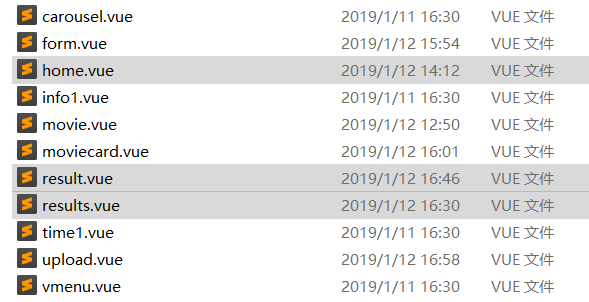
\includegraphics[width=0.5\linewidth]{images/components.png}
    \caption{组件列表}
    \label{fig:components}
\end{figure}

为了给予用户更好的体验,我们为页面设计了如下功能:

\begin{enumerate}
    \item 导航栏置顶。导航栏固定在顶部,且位于所有界面之上,方便用户在浏览到页面的任意位置时进行搜索以及返回主页面等跳转。
    \item 首页加入跑马灯。首页跑马灯推荐最近上映电影,通过点击可以跳转到对应的电影信息呈现界面。
    \item 图片搜索融入文字搜索框。图片搜索按钮与文字搜索框融合,将两搜索元素放在一起,而不是将其拆分放置于两处位置,从而使得页面更加简洁,搜索功能分布更加集中。
    \item 图片搜索优化。除了传统的点击上传,也支持拖拽上传;不仅支持针对电影海报的搜索,也可以针对预告片中的某一帧进行搜索,并且若进行预告片截图进行搜索,则跳转到该电影信息呈现界面的同时使预告片从该帧开始播放。
    \item 对于电影评论添加折叠按钮。可以方便的将选择显示或者隐藏电影评论,使得电影信息呈现界面更加清爽。
\end{enumerate}

\end{document}